%%%%%%%%%%%%%%%%%%%%%%%%%%%%%%%
\chapter{Simulation of proton-proton collisions}
\label{ch:dataAndSim}
%%%%%%%%%%%%%%%%%%%%%%%%%%%%%%%

The simulation of proton-proton collisions is usually performed by means of Monte Carlo (MC) event generators, providing an accurate modelling of the event kinematics and topology at parton and hadron level.
The hard inelastic scattering has to be fully calculated, namely, from the hard interaction between the partons inside the protons, where perturbative QCD calculations (\FIXME{ref}) can be used, to the formation of particle jets from the outgoing partons.
Furthermore, it is fundamental to understand the exact response of the detector to the outgoing particles produced in proton-proton collisions. 
Consequently, the stable outgoing particles are fed to a full detector simulation that models the interaction of those particles with the detector material and the corresponding detector response.
The raw detector data are then subject to the same reconstruction algorithms that are also used for real data.
In this chapter, MC event generators are described in detail, followed by a brief description of the CMS detector simulation.

%%%%%%%%%%%%%%%%%%%%%%%%%%%%%%%
\section{Monte Carlo event generators}
%%%%%%%%%%%%%%%%%%%%%%%%%%%%%%%

The generation of hard inelastic proton-proton collisions follows several steps depicted in Fig.~\ref{fig:MCgenSteps} and described in the following subsections.

\begin{figure}[!htb]
\centering
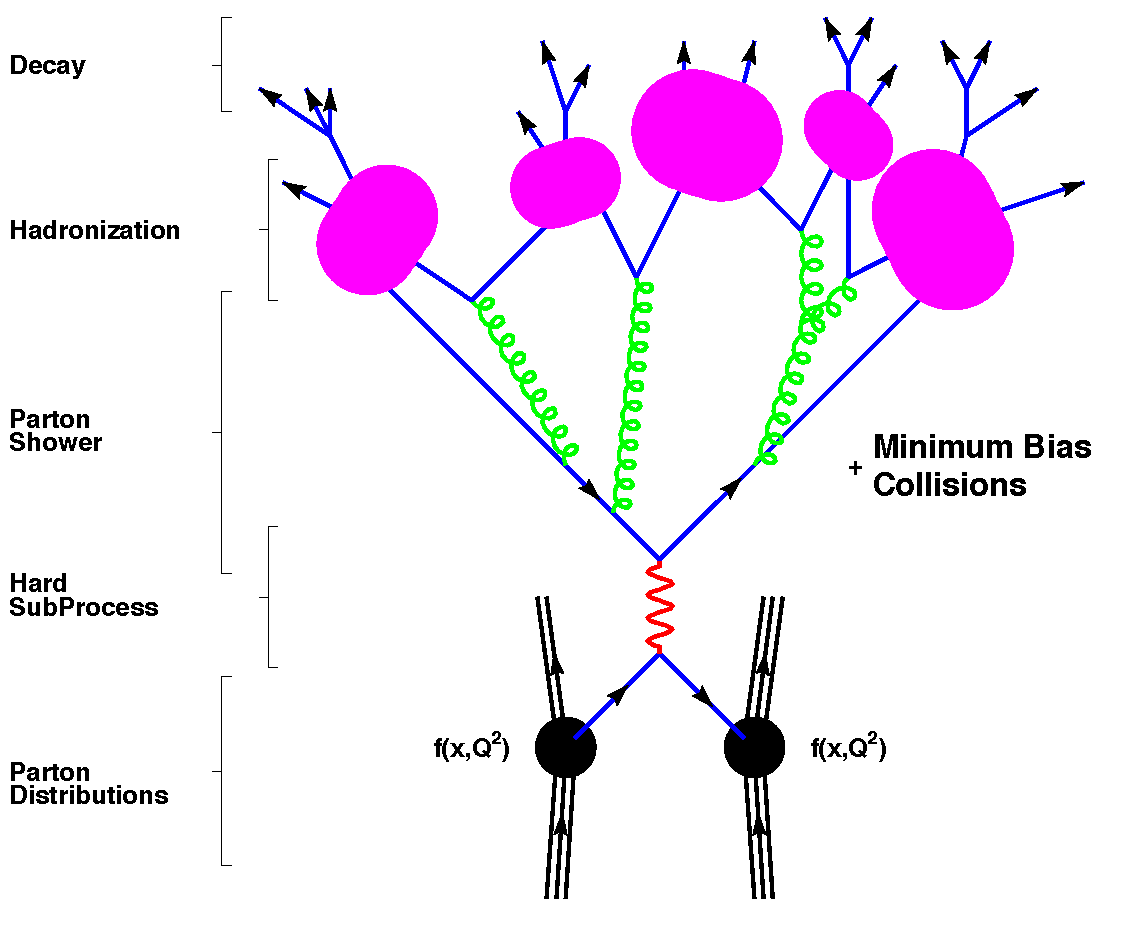
\includegraphics[width=0.8\textwidth]{\chfive/f_shg_event.pdf}
\caption{Steps of Monte Carlo event generation as described in the text evolving in time from bottom to top~\cite{Dobbs:2004qw}.}
\label{fig:MCgenSteps}
\end{figure}

\subsection{Hard process}

The basis of theoretical event generation at the LHC is a parametrisation of the incoming partons stemming from the proton, which is given by the parton density functions.
They describe the probability to find a quark or gluon within a given proton momentum fraction $x$ from the pp collision taking place at the LHC (\FIXME{ref}).
Using the incoming partons as input, the simulation of the hard process is performed by the event generator.
It produces hypothetical events with the distributions and rates predicted by theory based on the cross section formulae of the physics process of interest.

The cross section for the process is computed through a perturbative  approach.
In this approach where the matrix element between the initial state and a final state $X$ is computed as the sum of contributions with increasing powers of $\alpha_s$.
If $a$ and $b$ are the partons involved in the hard process part of the pp collision, the cross section associated to the process, $\sigma_{ab} \rightarrow X$, is derived.
For instance, the leading contribution to the W boson production process can be calculated from the diagram in Fig.~\ref{fig:wjets_LO}.
An accurate description of the process must however also take into account radiative corrections. They can be of two types: real (production of a quark or a gluon in addition to the W boson) or virtual (loop correction to the vertex or to the quark or antiquark propagator). The diagrams corresponding to the real corrections at the first order for W boson production are shown in Fig.~\ref{fig:wjets_NLO}.
Once the $\sigma_{ab} \rightarrow X$ partonic cross section is known, the total proton-proton cross section can be factorized according to the factorization theorem (\FIXME{ref}).

\begin{figure}[!htb]
\centering
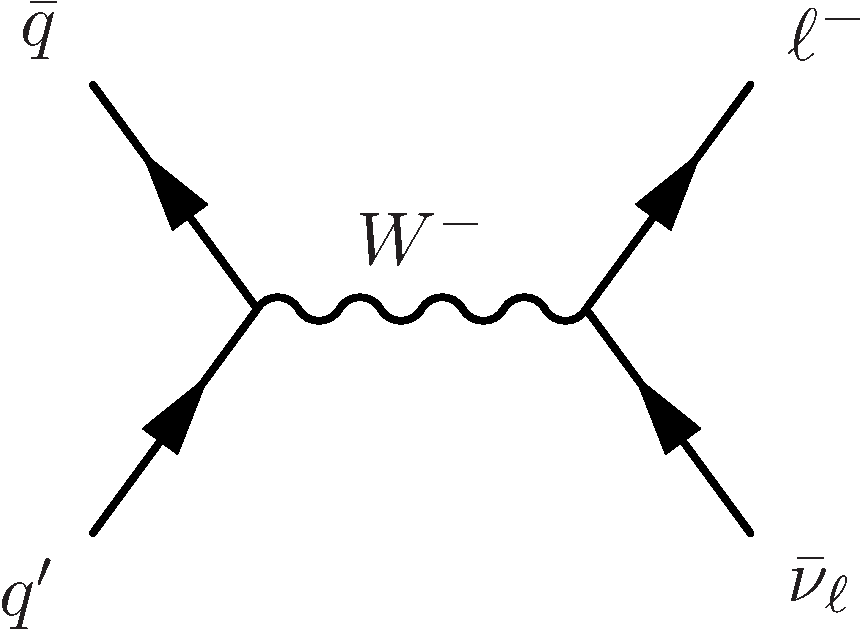
\includegraphics[width=0.3\textwidth]{\chfive/WplusJets_LO.pdf}
\caption{Feynman diagram contributing to the W boson production at leading order. The charge conjugate production mode is implied. Only the leptonic decay of the W boson is considered.}
\label{fig:wjets_LO}
\end{figure}

\begin{figure}[!htb]
\centering
\subfigure[]{\label{fig:wjets_NLO_a}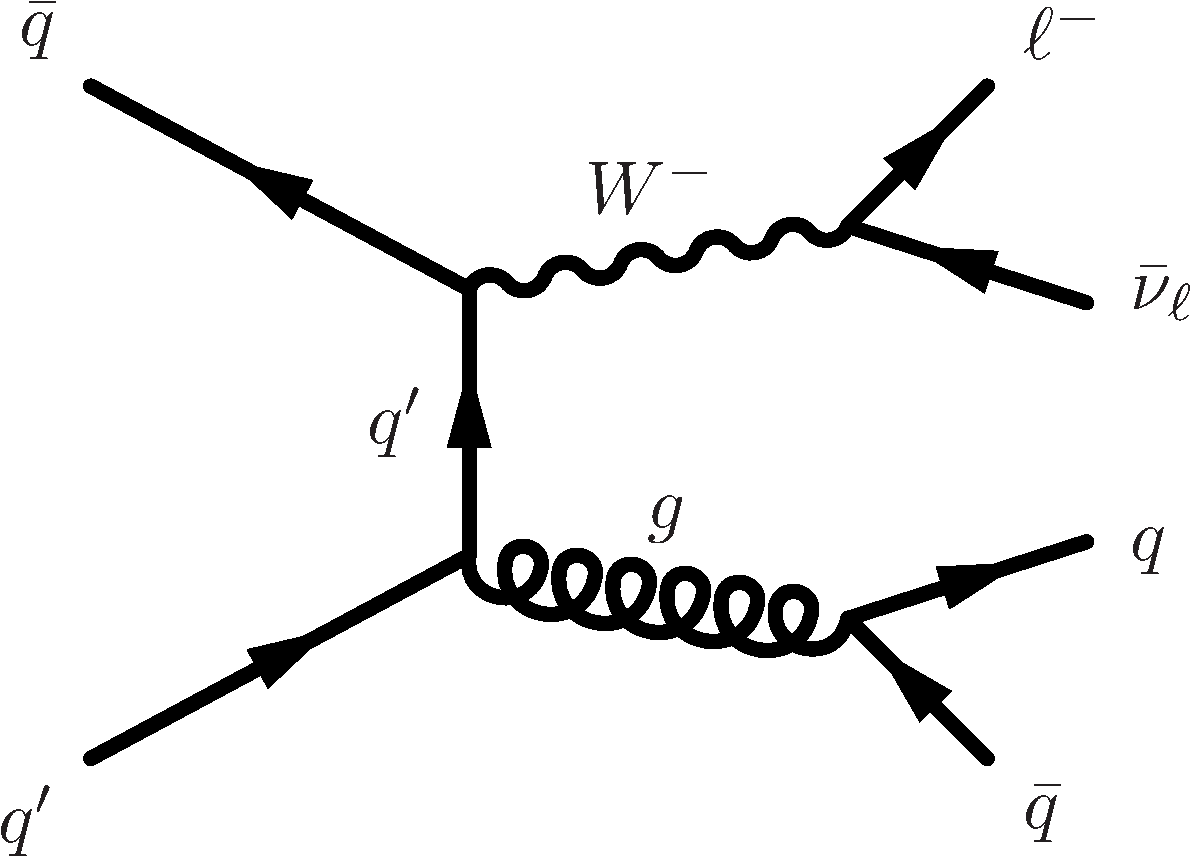
\includegraphics[width=0.3\textwidth]{\chfive/WplusJets_NLO_1.pdf}}
\subfigure[]{\label{fig:wjets_NLO_b}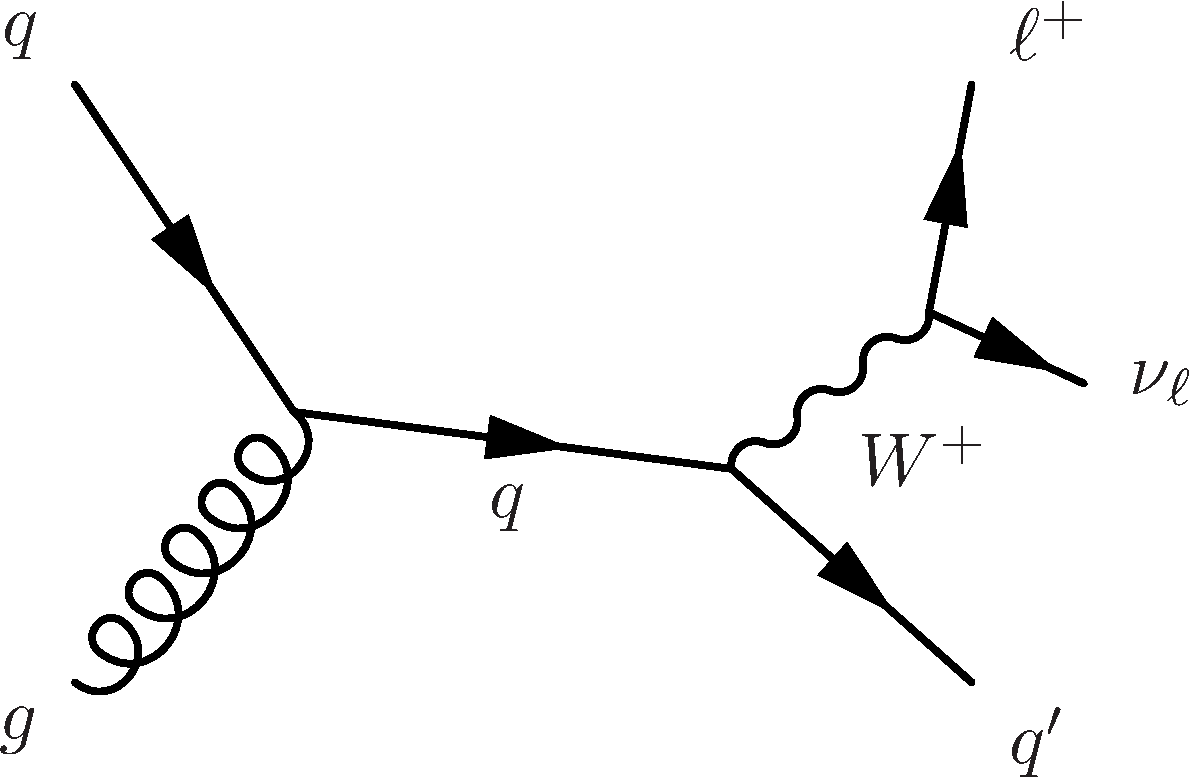
\includegraphics[width=0.3\textwidth]{\chfive/WplusJets_NLO_2.pdf}}
\caption{Feynman diagrams corresponding to the first order real radiative corrections to the W boson production in association with jets. The charge conjugate production modes are implied. Only the leptonic decay of the W boson is considered.}
\label{fig:wjets_NLO}
\end{figure}

Various generators are available to generate events according to a given hard process~\cite{Dobbs:2004qw}.
Although in principle all the orders of the perturbative development should be considered, most of them only include the leading contribution to the matrix element.
A popular generator is Pythia~\cite{Sjostrand:2007gs,Sjostrand:2006za}, a general purpose program which, in addition to the hard process, also takes care of the parton showering, the hadronisation, and the description of the underlying event.
For the matrix element calculation, Pythia only considers the leading order (diagram in Fig.~\ref{fig:wjets_LO} for the W production case).
The radiative corrections are not explicitily calculated but rather treated in the parton showering.
As will be discussed in the next section, the parton showering is well suited to treat low $Q^2$ radiation.
It however fails to accurately describe hard radiations. The consequence is that the performances of Pythia to describe events including many hard jets in the final state are limited.
A more accurate approach is followed by MadGraph~\cite{Alwall:2011uj} where the hard real radiative
corrections are included in the matrix element (Fig.~\ref{fig:wjets_NLO}). Diagrams with up to 5 extra partons are included. This generator is well suited to study processes such as W or Z produced in addition with hard jets.
Finally, the Powheg [96] generator is a complete next to leading order (NLO) generator that considers both real and virtual corrections at the leading order. It is therefore limited to the radiation of one hard extra parton after what it must rely on the parton showering description. The use of the full NLO nevertheless provides in general an accurate estimate of the inclusive cross section. Since the first parton radiation is already described, the interface between Powheg and the parton showering requires some special treatment.
In addition to event generators, there also exist cross section integrators which can be used to compute cross sections as a function of a variable of interest. An example is the FEWZ code [97] which allows one to make calculation at the NNLO level for exclusive production of a W or Z boson.

\subsection{Parton showering}

\subsection{Underlying event}

\subsection{Hadronization}

\subsection{Pileup}

\FIXME{Talk here about pileup simulation and re-weighting}

\begin{figure}[!htb]
\centering
\subfigure[]{\label{fig:pu_mc_data_a}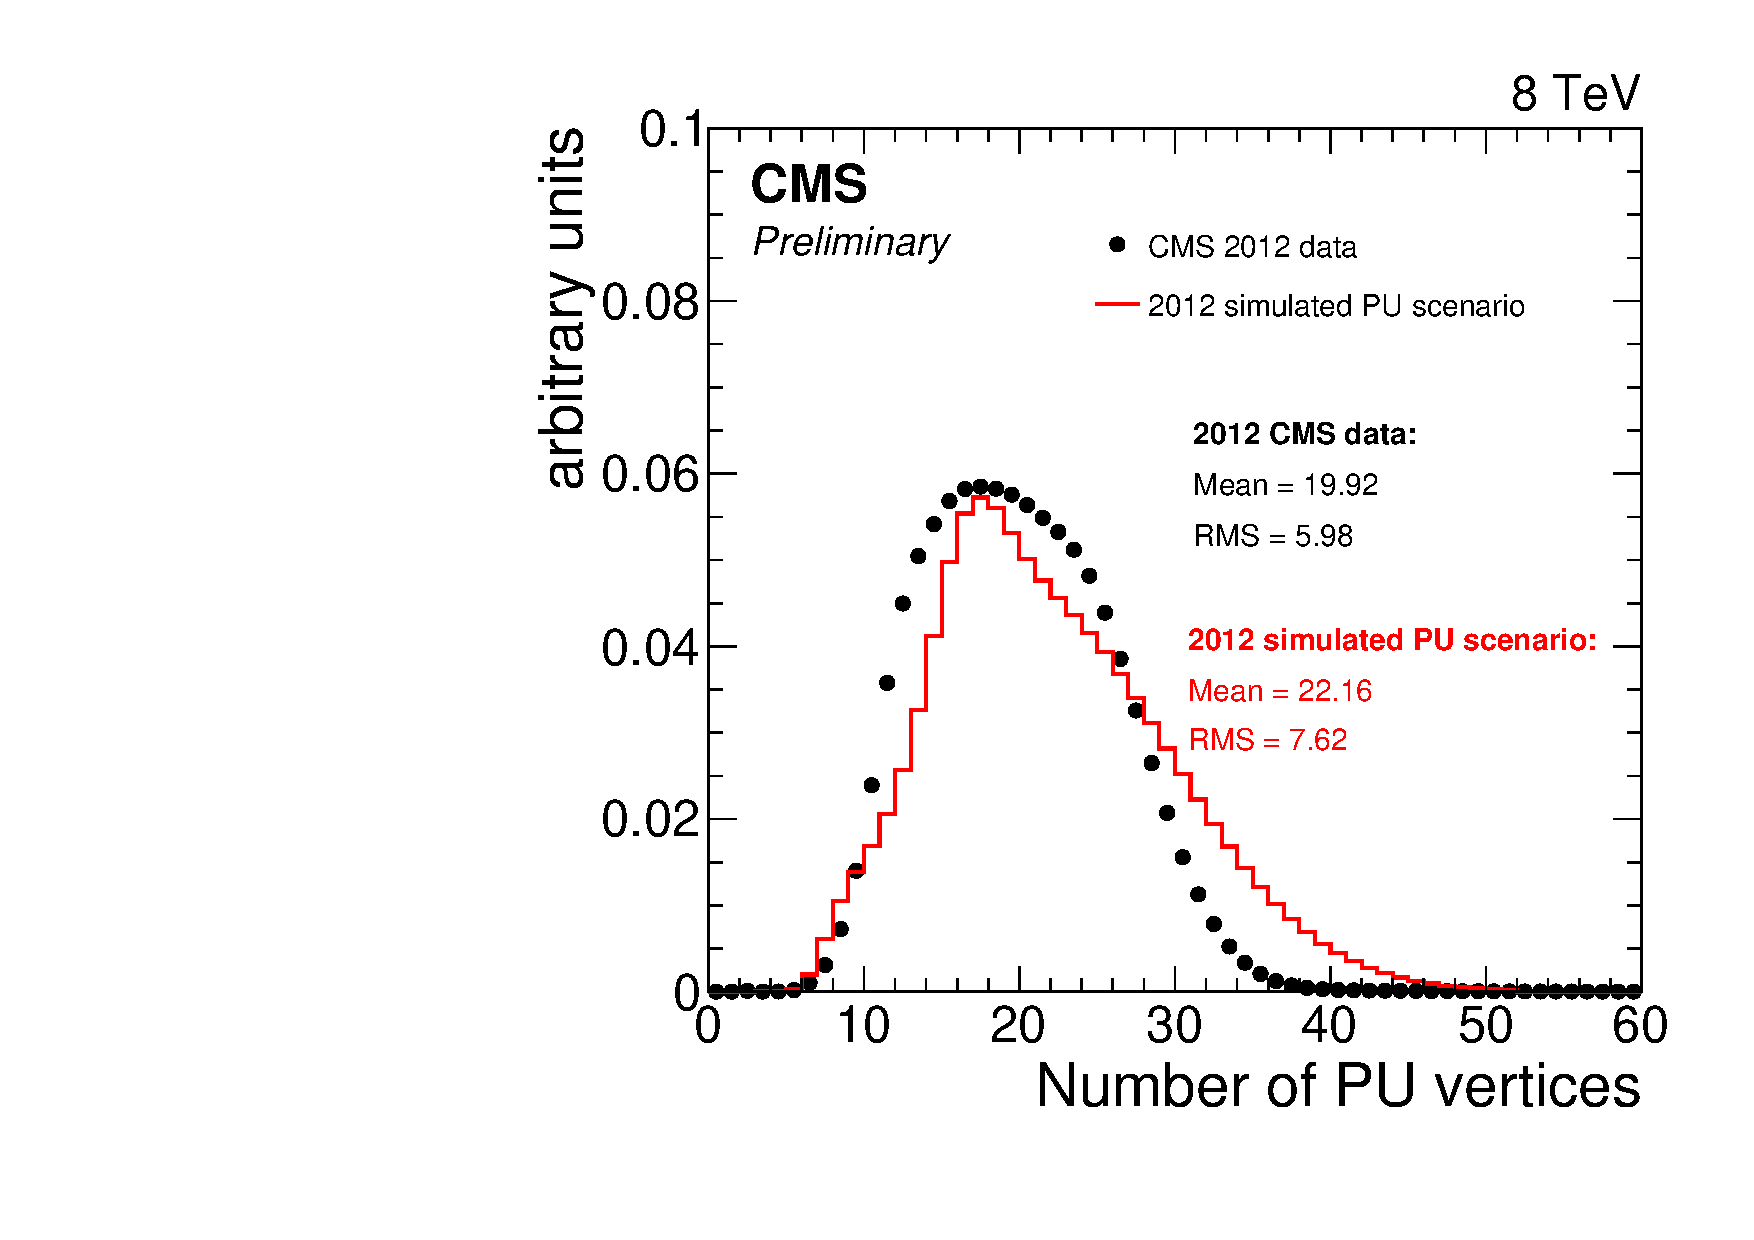
\includegraphics[width=0.45\textwidth]{\chfive/PU-data-mc-8TeV.pdf}}
\subfigure[]{\label{fig:pu_mc_data_b}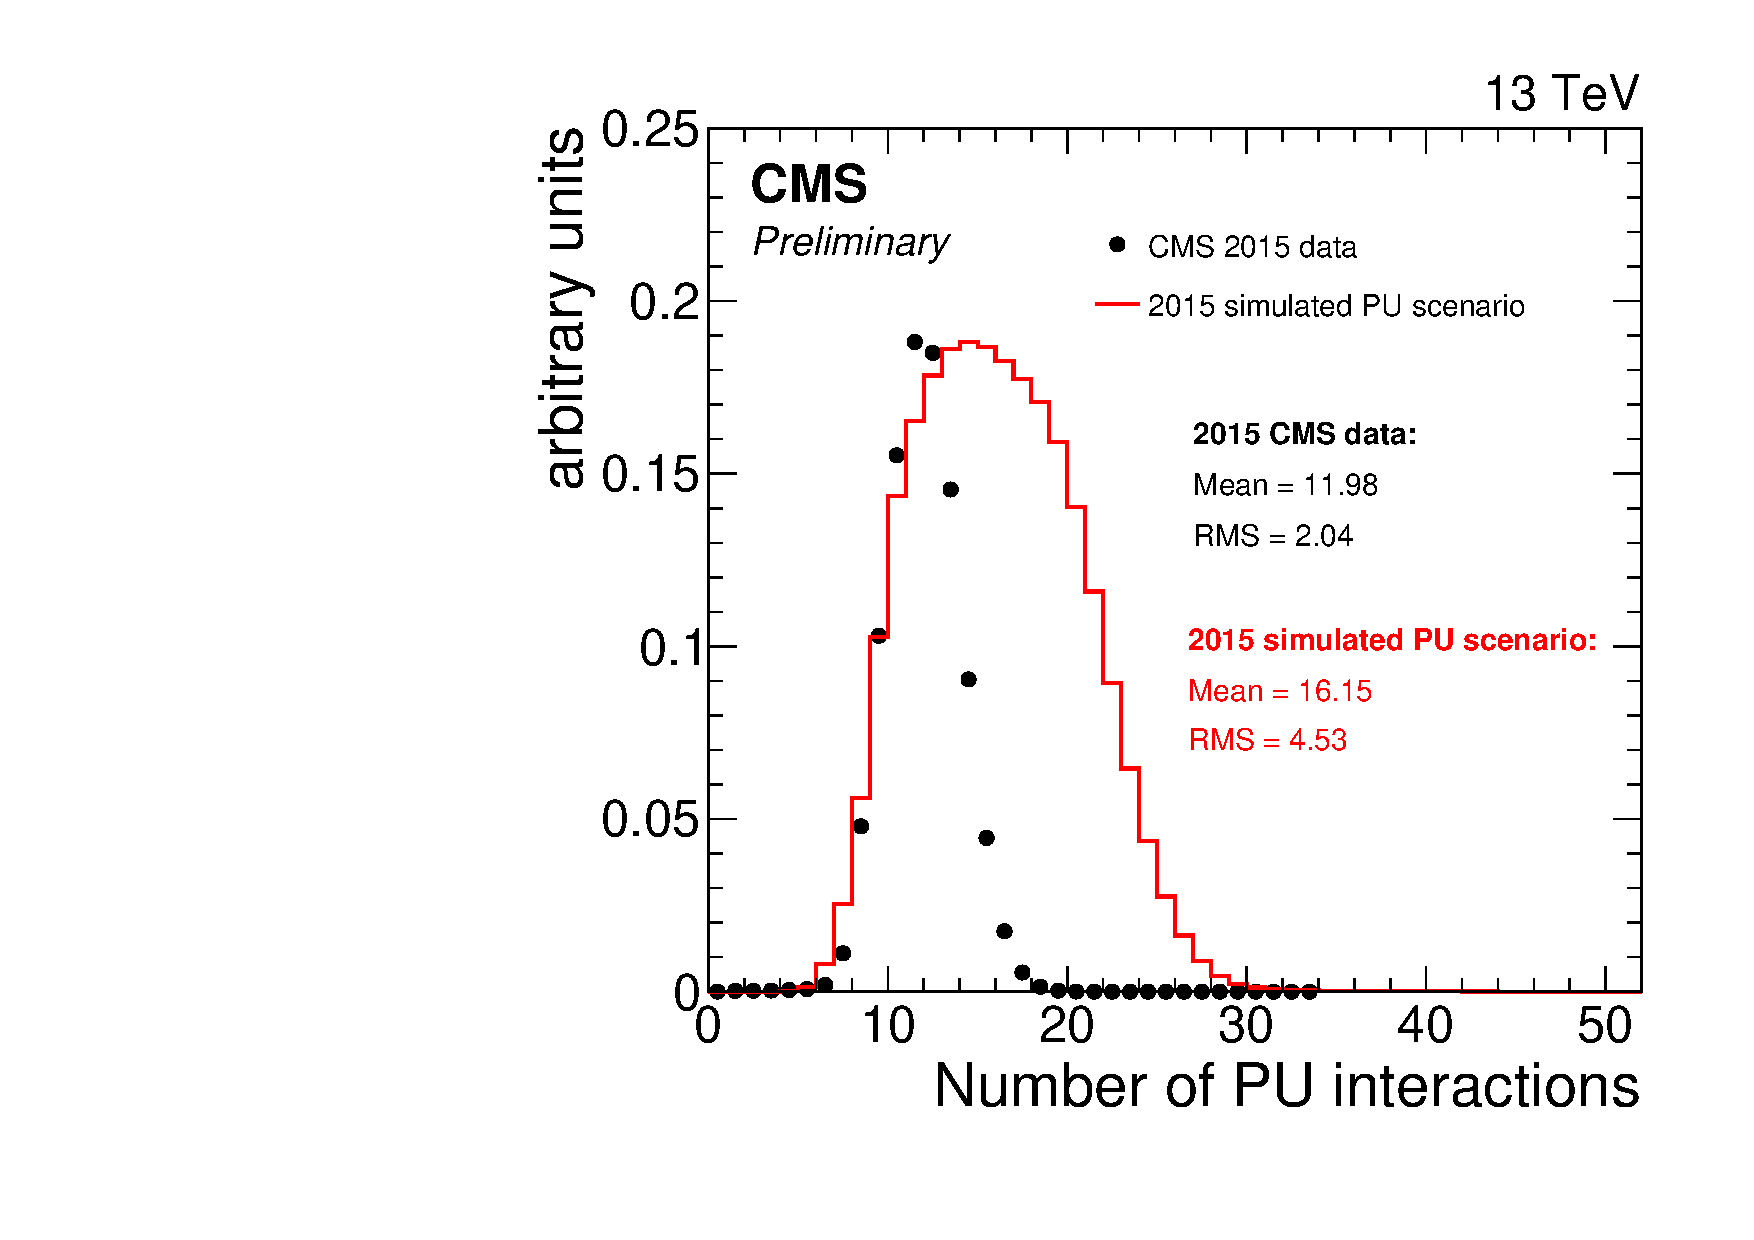
\includegraphics[width=0.45\textwidth]{\chfive/PU-data-mc-13TeV.pdf}}
\caption{blabla.}
\label{fig:pu_mc_data}
\end{figure}

%%%%%%%%%%%%%%%%%%%%%%%%%%%%%%%
\section{CMS detector simulation}
%%%%%%%%%%%%%%%%%%%%%%%%%%%%%%%

%%%%%%%%%%%%%%%%%%%%%%%%%%%%%%%
\section{Simulated samples}
%%%%%%%%%%%%%%%%%%%%%%%%%%%%%%%

\subsection{Simulation of signal processes}\label{subsec:signalMC}
\subsection{Simulation of background processes}
